\begin{figure}[htp] \centering
    \begin{subfigure}[b]{0.96\columnwidth}
        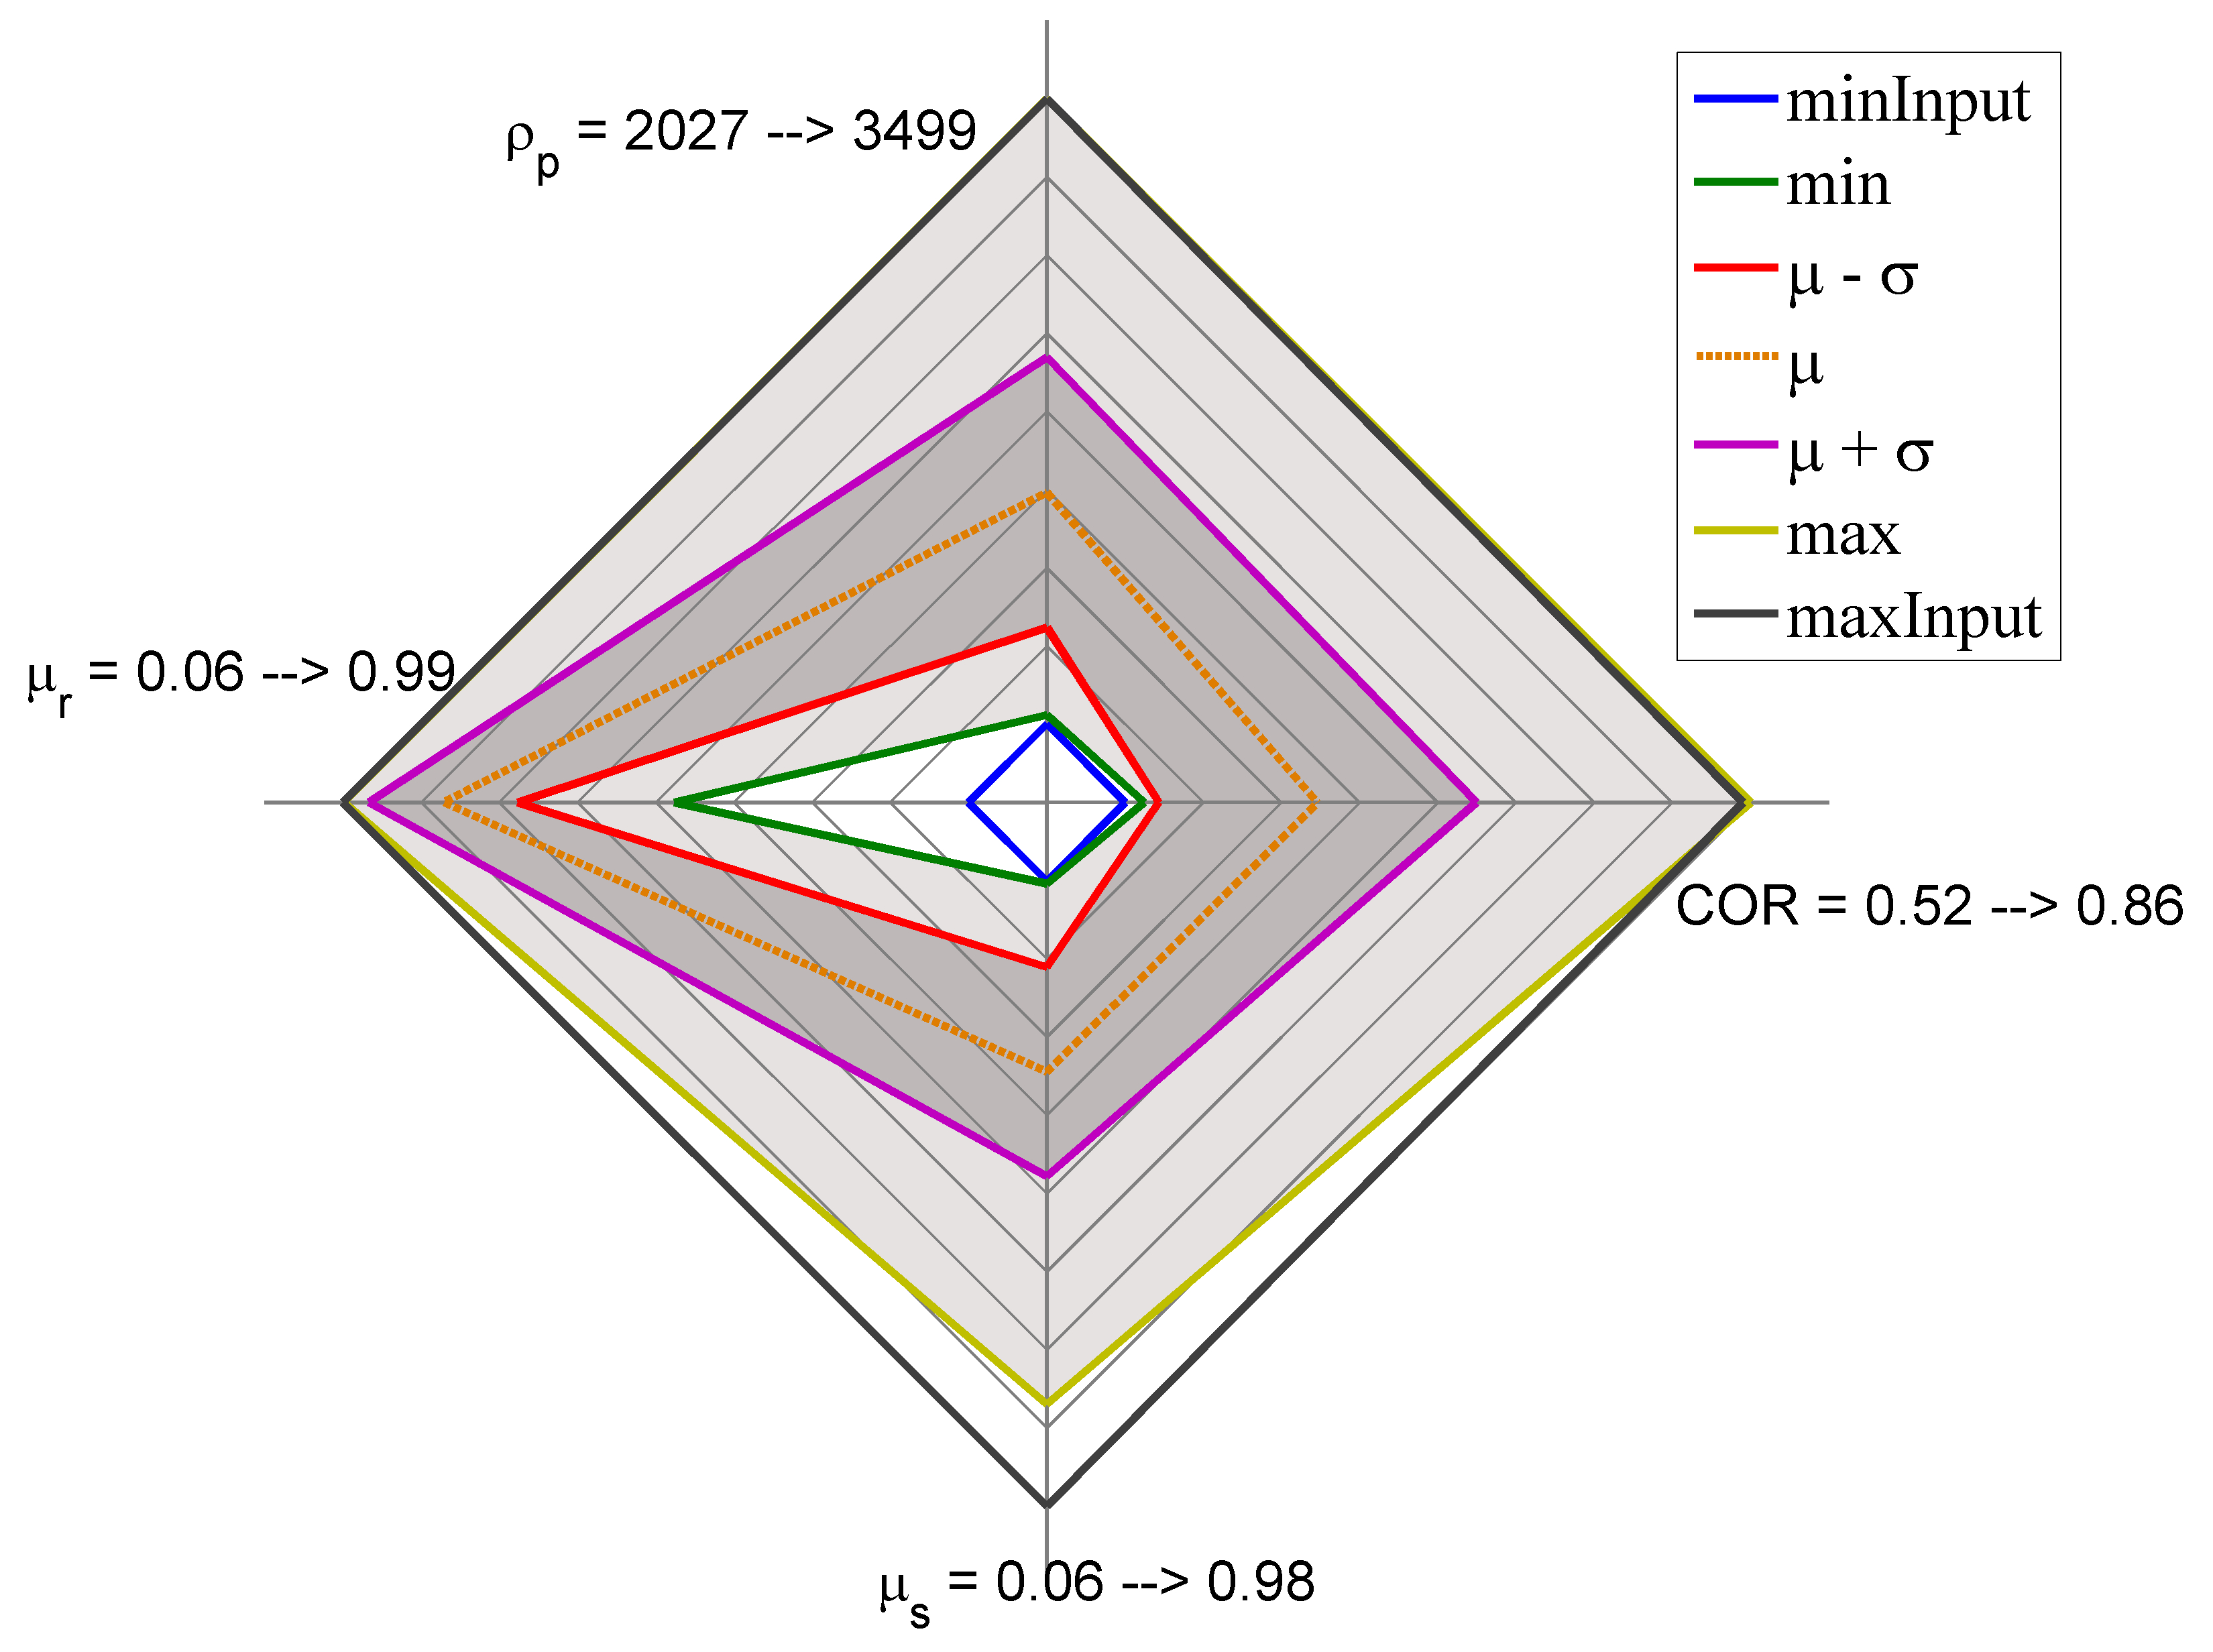
\includegraphics[width=\textwidth]{images/original/31radarpirker1aor}
        \caption{Radar plot, $AoR_{exp} = 38.85 ^\circ$}
        \label{fig:31radarpirker1aor} 
    \end{subfigure}\\
        \begin{subfigure}[b]{0.96\columnwidth}
        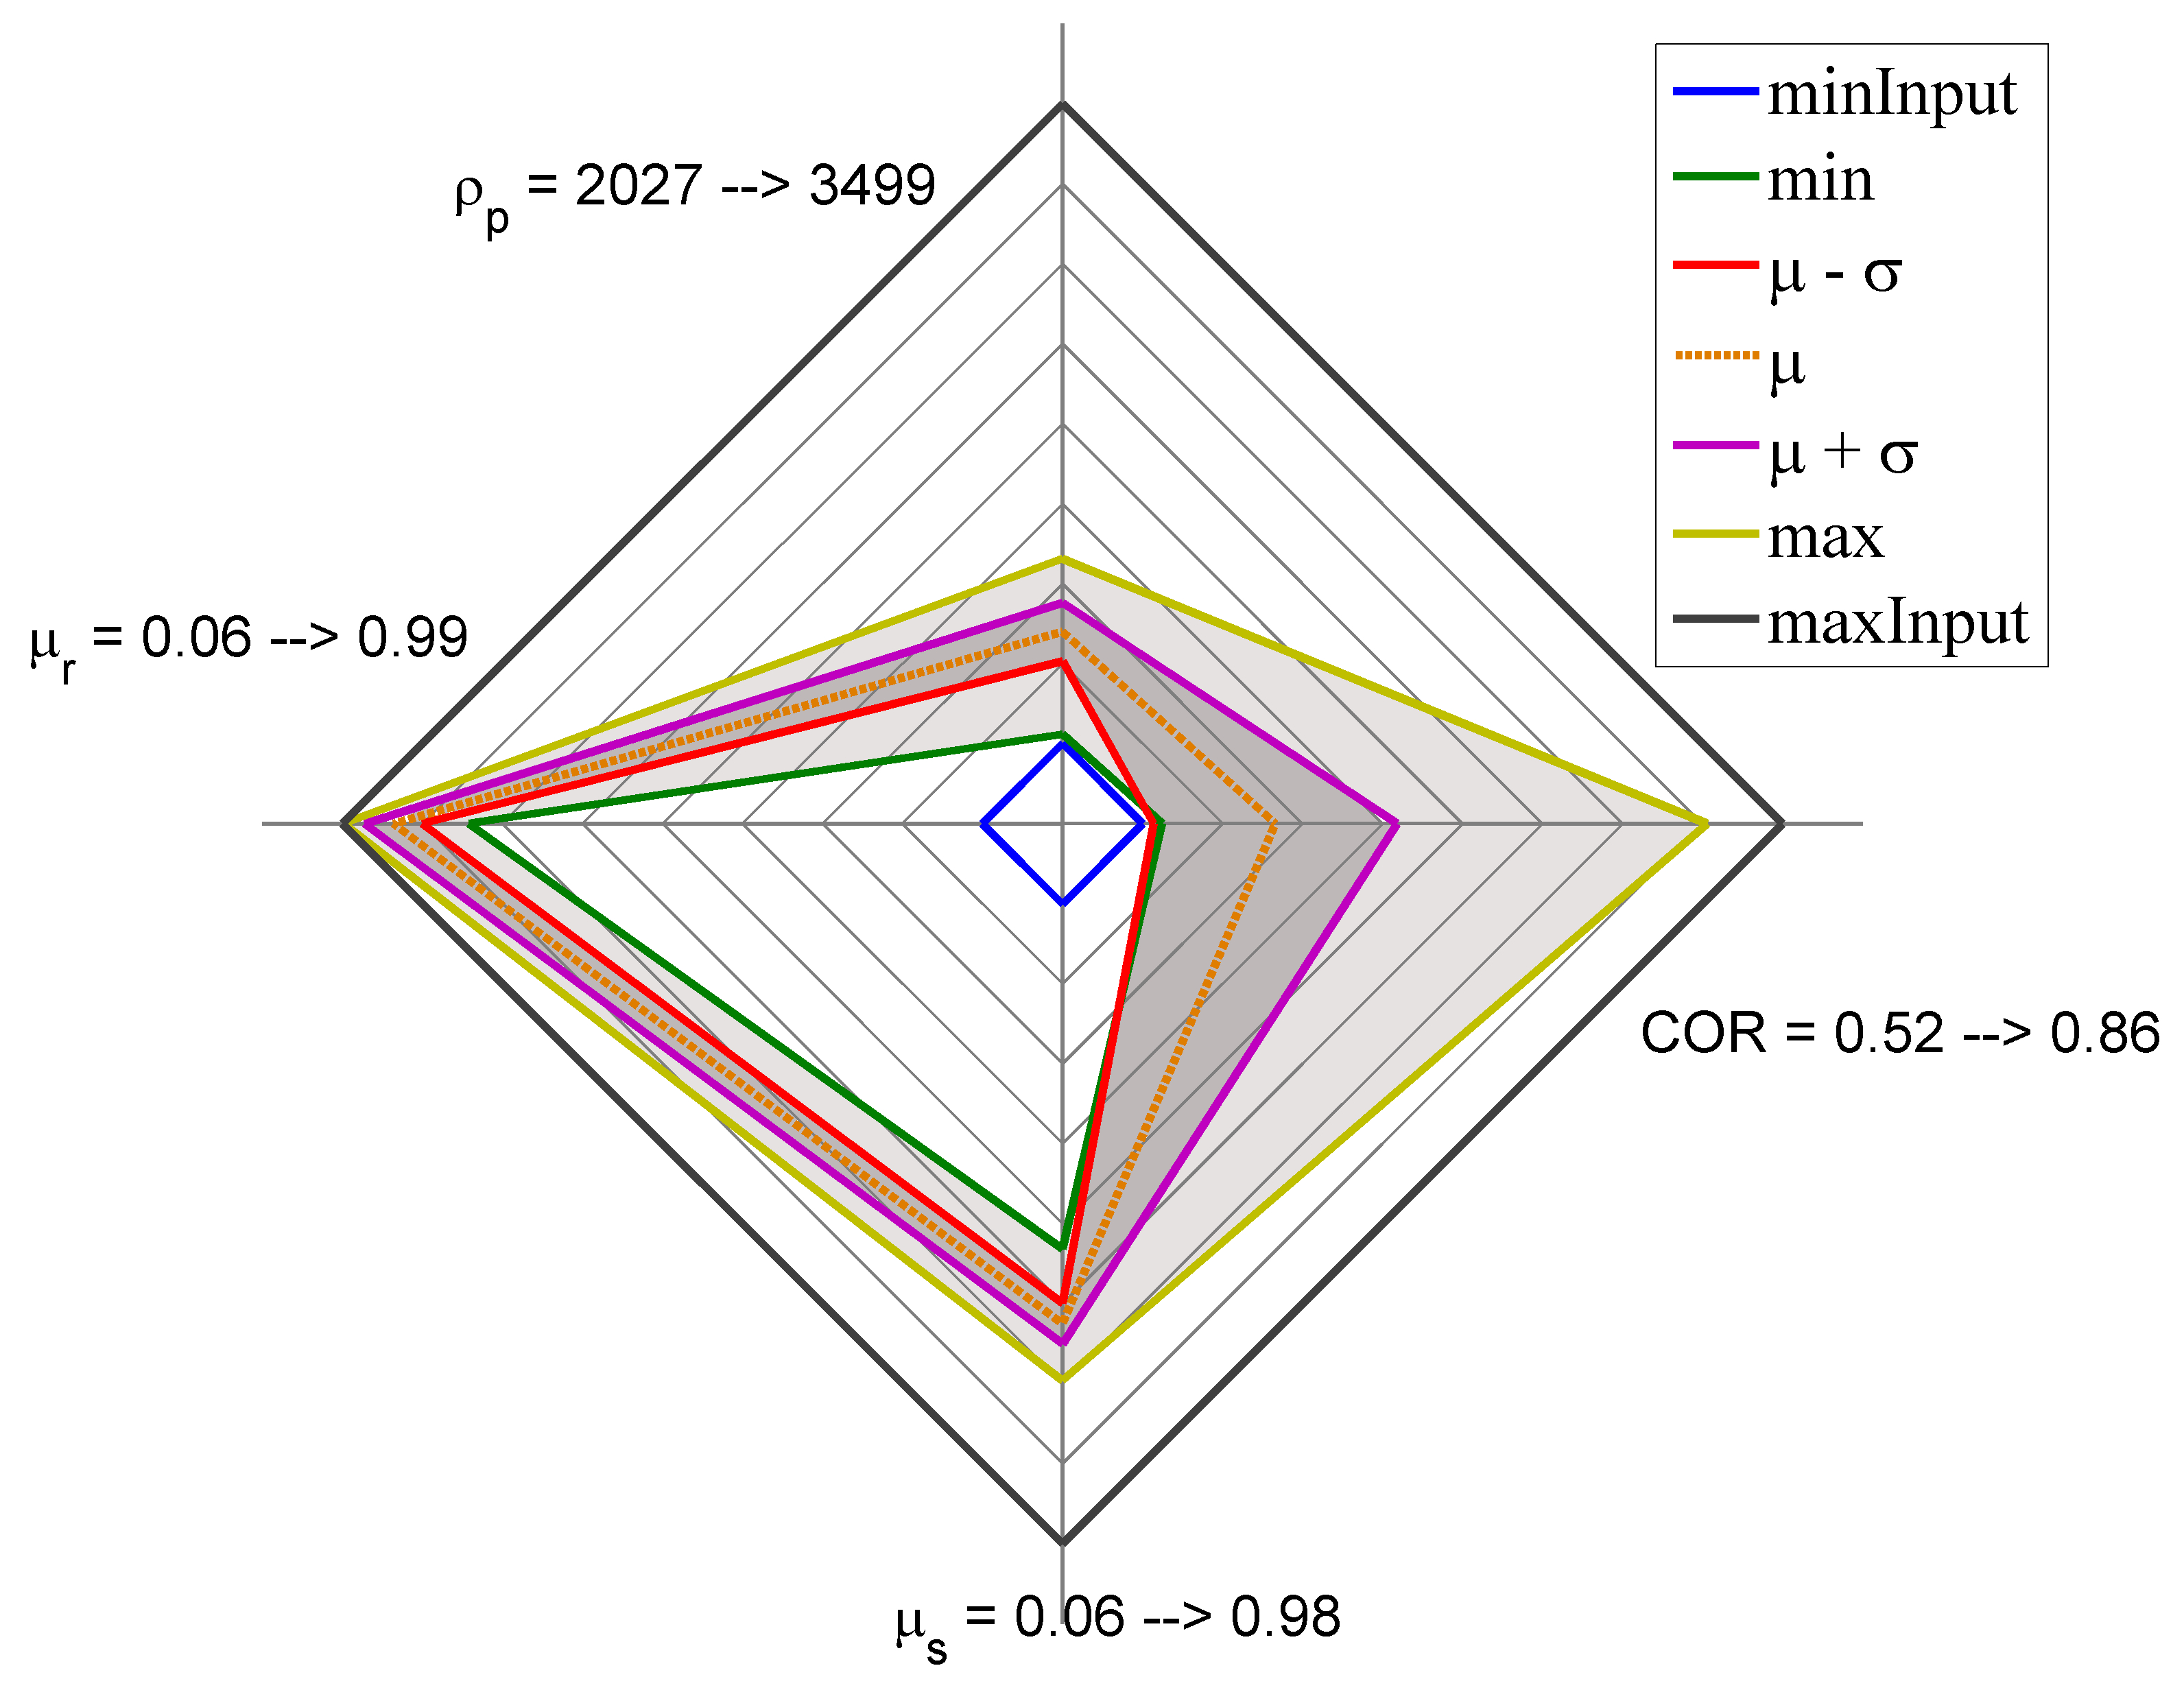
\includegraphics[width=\textwidth]{images/original/33radarpirker1schulze10070aor}
        \caption{Radar plot, $AoR_{exp} = 38.85
        ^\circ$ \& $SSC$: $\sigma_n=10070 ~[Pa]$}
        \label{fig:33radarpirker1schulze10070aor} 
    \end{subfigure}
    \caption[Radar plot of valid simulations parameters for the AOR and
    the merge between AOR and SCT valid parameters]{Radar plot of valid
    simulations parameters for the angle of repose tester ($AoR$) and the merge
    between AOR and shear cell tester ($SSC$).
    Each axes of the radar plot represents one simulation parameters.
    Furthermore, the shaded area represents valid parameters combinations.
    Dark shaded values stand for the confidence range.
    We represent the marked combinations for one load condition of the shear
    cell.
    Further explanation in the text. }
    \label{fig:35schulze10070aorradarandcloud}
\end{figure}